\documentclass[12pt]{article}
\usepackage[utf8]{inputenc}
\usepackage[T1]{fontenc}
\usepackage{amsfonts, amsmath, amssymb, amstext, graphicx, float, indentfirst, physics, listings}
% Please add the following required packages to your document preamble:
\usepackage{booktabs}
\usepackage[dvipsnames]{xcolor}
\usepackage{setspace} % Espaçamento 1.5
\usepackage[a4paper, top=3cm, bottom=2cm, left=3cm, right=2cm]{geometry} % Margens
\usepackage{hyperref}
\begin{document}

\begin{titlepage}
  \begin{center}
    \vspace*{1cm}
    \Huge{Estudo teórico-computacional da dinâmica de sistemas partículas-bolha aplicado em processos de flotação}

    \vspace{2cm}
    \Large{Prof. Dr. Petrus Henrique Ribeiro Anjos}

    \vspace{0.5cm}
    \Large{Me. Luis Vinicius Costa Silva}

    \vspace{0.5cm}
    \Large{Universidade Federal de Catalão - UFCAT}

  \end{center}
  
  
        \vfill
        
        Proposta de projeto de pesquisa para obtenção de bolsa de doutorado concedida pela FAPEG  Fundação de Amparo à Pesquisa do Estado de Goiás (FAPEG).
        
        \vspace{0.8cm}
          
  
\end{titlepage}

\pagenumbering{gobble} % Desabilita numeração de páginas

\newpage
\tableofcontents % Sumário

\newpage
\pagenumbering{arabic} % Ativa numeração de páginas
\doublespacing % Espaçamento 1.5

\section{Intodução e Justificativa}
Os métodos de Boltzmann em redes (Lattice Boltzmann - LB) ou modelos de Lattice Boltzmann (Lattice Boltzmann Method - LBM) são extremamente populares para modelar o fluxo e o transporte em escalas mesoscópicas de fluídos, onde nem modelos contínuos nem métodos de dinâmica molecular são práticos, e também para modelar fluxos contínuos em larga escala, onde métodos convencionais de Dinâmica dos Fluidos Computacional enfrentam dificuldades severas. O LBM foi escolhido como método de simulação neste trabalho devido a sua capacidade de capturar a mesma dinâmica modelada pelas equações de Navier-Stokes (como observado na expansão de Chapman-Enskog das equações em \cite{zhang2014lattice}), a facilidade na escrita do código e paralelização do mesmo em GPUs\cite{schlauch2013comparison}, e principalmente, em nosso caso, o acoplamento das equações governantes com fenômenos inerentes a dinâmica molecular relacionadas a composição química do fluído\cite{ning2016upscaling}.\newline

Além disso, o LBM simplifica a solução das equações de Navier-Stokes, que descrevem o movimento de fluidos, ao discretizar o espaço em uma grade regular e modelar o transporte de partículas através de colisões locais. Isso o torna particularmente eficaz para simular fluxos em geometrias complexas e para estudar fenômenos de transporte em fluidos complexos ou misturas de fluidos. Em comparação com métodos tradicionais de elementos finitos, o LBM oferece uma abordagem mais intuitiva e computacionalmente eficiente para modelagem de fluxo, especialmente em problemas com geometrias irregulares ou em movimento, como em processo de flotação em plantas de mineração.\newline


Em engenharia de minas, a flotação por espuma é um método altamente versátil para separar fisicamente partículas com base em diferenças na capacidade de bolhas de ar aderirem seletivamente a superfícies minerais específicas em uma suspensão mineral/água. As partículas com bolhas de ar aderidas são então levadas para a superfície e removidas, enquanto as partículas que permanecem completamente umedecidas ficam na fase líquida. Esse processo pode ser adaptado a uma ampla gama de separações minerais, pois é possível usar tratamentos químicos para alterar seletivamente as superfícies minerais, de modo a terem as propriedades necessárias para a separação. A flotação por espuma é utilizada em diversas aplicações, como separação de minerais de sulfeto da ganga de sílica e de outros minerais de sulfeto, separação de cloreto de potássio (silvita) do cloreto de sódio (halita), separação de carvão de minerais formadores de cinzas, remoção de minerais silicatos de minérios de ferro, separação de minerais de fosfato de silicatos, e até mesmo em aplicações não minerais, como em tratamento de água. É particularmente útil para processar minérios de grão fino que não são adequados para concentração por gravidade convencional.\newline

Um processo de flotação depende fundamentalmente de três grandes elementos, são eles:


\begin{itemize}
    \item Componentes Químicos
    \begin{itemize}
        \item Coletores
        \item Espumantes
        \item Ativadores
        \item Depressores
        \item pH
    \end{itemize}
    \item Componentes de Equipamento
    \begin{itemize}
        \item Design da Célula
        \item Agitação
        \item Fluxo de Ar
        \item Configuração do Banco de Células
        \item Controle do Banco de Células
    \end{itemize}
    \item Componentes de Operação
    \begin{itemize}
        \item Taxa de Alimentação
        \item Mineralogia
        \item Tamanho de Partícula
        \item Densidade da Polpa
        \item Temperatura
    \end{itemize}
\end{itemize}


É importante levar em conta todos esses fatores acima nas operações de flotação por espuma, não apenas para entender a dinâmica do sistema estudado, mas para aprimora-lo. Mudanças nas configurações de um fator, como taxa de alimentação, automaticamente causarão ou demandarão mudanças em outras partes do sistema, como taxa de flotação, recuperação de tamanho de partícula, fluxo de ar, densidade de polpa, etc. Como resultado, é difícil estudar os efeitos de qualquer fator isoladamente, e os efeitos de compensação dentro do sistema podem impedir que as mudanças no processo produzam os efeitos esperados. Isso torna difícil desenvolver modelos preditivos para flotação por espuma, embora trabalhos estejam sendo realizados para prever o desempenho do circuito a partir de parâmetros facilmente mensuráveis, como recuperação de sólidos e teor sólido de rejeitos\cite{chen2020lattice,karimi2014cfd,michaux2018challenges}, apesar de que os trabalhos desenvolvidos até o momento não apresentam resultados conclusivos por estarem em um estágio incipiente.



Devido a importância econômica do processo de flotação, um grande esforço de pesquisa tem sido feito para aumentar sua eficiência através de um melhor entendimento da física subjacente ao processo \cite{ives2012scientific}. Abordagens numéricas em escala macroscópica foram propostas e utilizadas para analisar fenômenos de fluxo de fluidos multicomponentes, como como método do volume de fluido \cite{hirt1981volume}, rastreamento frontal \cite{tryggvason2001front} e interface difusa \cite{anderson1998diffuse}. Na escala mesoscópica, o método da rede de Boltzmann (LBM) \cite{he1997theory} tem sido considerado devido às suas diversas vantagens sobre dinâmica de fluidos computacional clássica (CFD) \cite{kruger2017lattice}, como facilidade de implementação, paralelismo e manipulação de geometrias complexas. Em uma escala mcroscópica, métodos de dinâmica molecular \cite{xia2020role} tem sido utilizados para simular e esclarecer os mecanismos de ligação partícula-bolha \cite{foucaud2019review} e predição de reagentes para flotação \cite{abdalla2018prediction}.

Apesar de todo esforço de pesquisa feito até aqui a implementação de modelos computacionais para simulação de fluxos de fluidos com três ou mais componentes ainda tem diversos perguntas em aberto. Em particular o comportamento desses sistemas quando sujeitos a forças de flutuação e arrasto tem se provado difícil devido a instabilidades numéricas \cite{ghorbanpour2020numerical}. \newline

Assim, este trabalho busca compreender a dinâmica de escoamento e molecular em um processo de flotação para um melhor gerenciamento do processo e aprimoramento do mesmo, seja através de uma otimização de forma do design da célula/coluna de flotação, a sintetização de moléculas para reagentes/depressores, desenvolvimento de novos equipamentos e procedimentos, etc.

\section{Objetivos}
A dinâmica dos modelos multifásicos desempenha um papel importante em muitos campos da ciência e engenharia aplicadas, incluindo o fluxo de óleo-água-ar em meios porosos, a solidificação de ligas metálicas e a fusão de sólidos em presença de um líquido. Tipicamente, os modelos multifásicos manifestam uma ampla variedade de padrões geométricos (ou regimes de fluxo) das fases associadas, dependendo das condições do sistema. Esses padrões incluem, mas não se limitam a, fluxos com bolhas, de lama, de vórtice, anulares e também podem envolver interfaces triplo (três fases).\newline

Esses múltiplos padrões de fluxo afetam significativamente a hidrodinâmica geral do sistema, variando as características de transferência de calor e queda de pressão de um determinado fluxo.\newline

Devido à existência de diferentes regimes de fluxo e suas transições temporais e espaciais locais (dependendo das condições locais do sistema), a modelagem preditiva se torna difícil e desafiadora. A simulação e identificação desses regimes de fluxo através da resolução de interfaces via simuladores tradicionais baseados em Navier-Stokes (N-S) são computacionalmente complexas, extremamente demoradas e frequentemente muito ineficientes, em parte devido à necessidade de um extenso rastreamento de interfaces. \newline
Além disso, como as interfaces entre as fases de um sistema multifásico são resultados de efeitos termodinâmicos únicos, também é necessário conhecer a equação de estado governante para incorporar uma termodinâmica consistente que geralmente é desconhecida nas regiões interfaciais. Consequentemente, as análises de modelos multifásicos ainda são amplamente baseadas nas correlações empíricas desenvolvidas para diferentes regimes de fluxo.\newline
Este trabalho tem como objetivo analisar o processo de flotação por meio de modelos de rede de Boltzman e investigar os efeitos de diferentes parâmetros sobre a eficiência do sistema. Mais detalhadamente:

\begin{enumerate}
    \item Implementar simulações de diferentes modelos de Rede de Boltzman para fluidos multifásicos, a saber: método do gradiente de cor\cite{gunstensen1991lattice}, método de pseudopotenciais \cite{shan1993lattice}, método das energias livres \cite{swift1996lattice}, método do campo de fases \cite{he1999lattice}.
    \item Comparar os métodos implementados para diferentes razões de densidade, viscosidade e fluxo de velocidade.
    \item Comparar os métodos implementados apartir de alguns {\it benchmarks}: (a) Espalhamento de lente líquida \cite{craster2006dynamics}, (b) 
    Instabilidade de  Rayleigh-Taylor \cite{sharp1984overview}, (c) Dinâmica de Bolhas ascendentes \cite{wang2018bubble}.
    \item Investigar os efeitos do diâmetro das bolhas, diâmetro das partículas no processo.
    \item Investigar os efeitos da tensão superficial no processo.

    \item Investigar o uso de métodos de dinâmica molecular para gerar, a partir de uma simulação microscópica, os parâmetros da simulação em escala mesoscópica.

Técnicas de DFT e dinâmica molecular serão utilizadas para compreender o comportamento a nível molecular dos compostos inseridos no processo, através do uso das equações de Cahn-Hillard e equação de Schrodinger acopladas ao modelo LBM.\newline

Adicionalmente, busca-se estudar e se possível aprimorar o algoritmo Watershed \cite{peng2021bubble,jahedsaravani2017image} para validação das simulações numéricas que descrevem a dinâmica do sistema em questão. Em síntese, uma vez que um modelo matemático é derivado à partir de observações do sistema físico (e alguns pressupostos/ansatz), simulações numéricas e resoluções analíticas serão desenvolvidas para capturar e compreender a dinâmica do sistema. Estas simulações por sua vez serão validadas através de técnicas de visão computacional, utilizando redes neurais e o algoritmo Watershed.
   
\end{enumerate}

\section{Metodologia}
\subsection{Softwares e bibliotecas utilizadas}
Códigos nativos serão escritos em Python utlizando bibliotecas como Fenics (para resolução de EDPS)\cite{barrata2023dolfinx}, PyClaw (resolução de EDPS hiperbólicas)\cite{ketcheson2012pyclaw} assim como as bibliotecas usuais para computação científica como Numpy, Scipy, Matplotlib, etc. Adicionalmente a biblioteca OpenLB\cite{kummerlander2023openlb} será utilizada para casos onde não será necessário escrever um solver dos primeiros príncipios. Esta biblioteca possui uma série de solvers derivados do LBM, assim como rotinas que facilitam a implementação de cenários mais complexos, permitindo o fácil carregamento de modelos 3D, uso de multimalhas adaptativas, computação distribuída, checkpoints para gravação de resultados, etc.\newline
Ademais, para pós-processamento e visualização de resultados será utilizado o software Paraview\cite{ahrens200536}, que possibilita trabalhar com grandes conjuntos de dados científicos em 3D, gerados pelas simulações numéricas citadas anteriormente, incluindo aquelas realizadas na área de Dinâmica dos Fluidos Computacional (CFD). Ele oferece uma variedade de recursos poderosos para visualização interativa, como renderização de alta qualidade, ferramentas de análise de dados, capacidade de lidar com conjuntos de dados distribuídos e a capacidade de visualizar e analisar dados em tempo real.
\subsection{Instalações de teste}
Ensaios de flotação e outros experimentos serão realizados no  Laboratório de Modelamento e 
Pesquisa em Processamento Mineral (LaMPPMin), associado a UFCAT. O laboratório possui uma míriade de equipamentos, como uma Célula de Flotação de Bancada 
Denver CFB-1000 - CD, necessária para elaboração de experimentos de flotação, balanças semi-
análiticas para pesagem de materiais e agitadores para misturas de compostos, caixa de bomba com 
bomba de polpa centrífuga (para bombeamento da polpa até a célula e etc. Uma descrição detalhada 
das instalações do laboratório estão disponíveis em \href{http://pnipe.mcti.gov.br/laboratory/3156}{http://pnipe.mcti.gov.br/laboratory/3156}
\subsection{Laboratórios computacionais}
A UFCAT possui o Laboratório Multiusuário de Computação de Alto Desempenho (LaMCAD) que será utilizado, se necessário, para executar as simulações de escoamento de fluido delineadas no projeto e processamento de dados relacionados. O Laboratório LaMCAD da UFCAT é um ambiente de computação de alto desempenho (HPC) com clusters. Ele possui um nó principal e vários nós de computação com diferentes configurações de hardware, incluindo CPUs Intel e AMD, memória RAM e armazenamento. No total, o LaMCAD possui 1828 núcleos de processamento, 7 TB de RAM e 288 TB de armazenamento, todos interconectados por uma rede Infiniband de 100 Gbps. Além disso, o laboratório conta com o ambiente CEMPA, que possui 704 núcleos, 2,88 TB de RAM e 165 TB de armazenamento dedicados.\newline 
Uma descrição detalhada  das instalações do laboratório estão disponíveis em \newline \href{https://lamcad.ufg.br/p/32808-infraestrutura-e-capacidade-computacional}{https://lamcad.ufg.br/p/32808-infraestrutura-e-capacidade-computacional}.\newline
Ademais, o \href{https://dccat.catastronomy.com/press.html}{Departamento Computacional Catastronomy (DCCat)} é um novo laboratório na Universidade Federal de Catalão que está sendo implantado e poderá ser utilizado à medida que este é colocado em funcionamento.
\subsection{Métricas de performance}
\subsubsection{Avaliação do processo de flotação experimental}
As métricas de avaliação utilizadas para mensurar a performance de cada processo experimental de flotação serão a razão de concentração, recuperação de metal, recuperação de peso e razão de enriquecimento. Uma vez que não existe uma métrica universal capaz de aferir absolutamente a performance do processo, cada uma será utilizada de acordo com o contexto dos experimentos desenvolvidos.\cite{kawatra2011fundamental}
\begin{enumerate}
\item \textbf{Razão de Concentração}:
A Razão de Concentração é dada por $F/C$, onde $F$ é o peso total da alimentação e $C$ é o peso total do concentrado. Também pode ser expressa em termos de teores de minério. Começando com as equações de balanço de massa e a definição da razão de concentração:
\begin{align*}
F &= C + T, & Ff &= Cc + Tt, & \text{Razão de Concentração} &= \frac{F}{C}
\end{align*}
onde $F$, $C$ e $T$ são os pesos da alimentação, concentrado e rejeitos, respectivamente; e $f$, $c$ e $t$ são os teores da alimentação, concentrado e rejeitos. Eliminando $T$ dessas equações temos:

\begin{equation}
\frac{F}{C} = \frac{c - t}{f - t}
\end{equation}

\item \textbf{Recuperação de Metal}:
Recuperação de Metal é a porcentagem do metal na alimentação original que é recuperada no concentrado. Pode ser calculada usando pesos e teores como $\left(\frac{Cc}{Ff}\right) \times 100$. Alternativamente, pode ser calculada apenas com os teores usando $\frac{100(c/f)(f - t)}{c - t}$.

\item \textbf{Perda de Metal}:
Perda de Metal representa o material perdido para os rejeitos e é simplesmente $100 \%$ menos a Recuperação de Metal.

\item \textbf{Recuperação de Peso}:
Recuperação de Peso é o inverso da Razão de Concentração e equivale a $100 \times \frac{C}{F} = 100 \times \frac{f - t}{c - t}$.

\item \textbf{Razão de Enriquecimento}:
A Razão de Enriquecimento é calculada diretamente a partir dos teores como $c/f$, sem envolver pesos no cálculo.
\end{enumerate}
\subsubsection{Avaliação dos resultados numéricos}
A acurácia e performance do LBM foi avaliada através de alguns casos-teste com resultados amplamente conhecidos na literatura, foram eles: escoamento de Poiseuille, escoamento na cavidade com tampa móvel,\cite{chen1996boundary} teste de bolha estática e simulações multibolha \cite{gupta2007lattice,jones1975interrelation,takada2001simulation}. Ademais, as seguintes métricas usuais serão utilizadas para validação de experimentos\cite{oberkampf1994proposed}: 

\begin{enumerate}
    \item Análise do Número de Courant-Friedrichs-Lewy (CFL);
    
    \item Critério de Convergência;
    
    \item Expoente de Lyapunov;
        \item Erro Médio Quadrático (MSE);
    
    \item Erro Relativo (\%);
    
    \item Coeficiente de Correlação ($R^2$);
    
    \item Erro de RMS (Root Mean Square);
    
    \item Erro de Medição (ME);
\end{enumerate}



\section{Resultados Esperados}
Espera-se que ao fim deste projeto, um modelo computacional seja desenvolvido e validado, de tal forma que os processos termodinâmicos e de escoamento inerentes a flotação sejam bem compreendidos assim como as variáveis de projetos das equações governantes, permitindo um aprimoramento do processo em questão.\newline
Adicionalmente, uma série de técnicas teórico-computacionais e resultados experimentais serão desenvolvidos para que tal objetivo seja alcançado, e estas são também um produto deste projeto. Logo, as publicações de artigos abrangerão desde uma revisão/survey sobre os aspectos teórico-computacionais dos fenômenos físico-químicos relacionados a flotação, desenvolvimento de técnicas computacionais para tratamento do problema, procedimentos para realização de experimentos e melhoramento do processo de flotação.\newline
Na eventualidade do desenvolvimento de um novo produto como um reagente, depressor, coluna de flotação, programa de computador, uma patente poderá ser registrada para viabilizar o uso comercial do produto desenvolvido.
\section{Cronograma}
O diagrama de Gantt abaixo ilustra como as atividades principais delineadas para a condução do projeto estão distribuidas ao longo de um período de 48 meses, considerando a entrada no programa em outubro de 2023 e uma defesa da tese e conclusão do doutorado em outubro de 2027.


\begin{figure}[H]
    \centering
    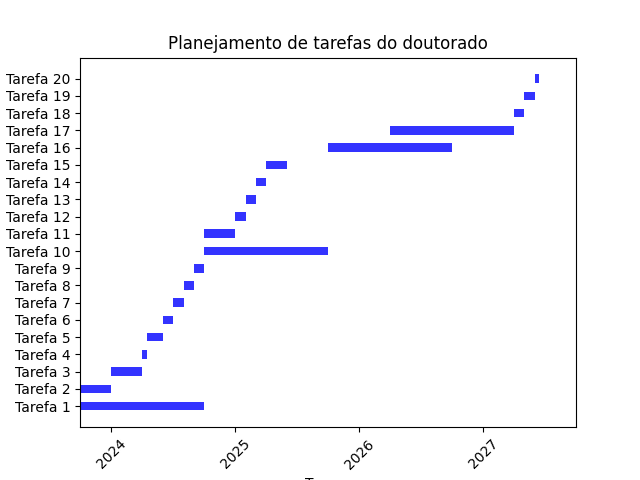
\includegraphics[width=\textwidth]{cronograma.png}
    \caption{Cronograma das atividades do doutorado}
    \label{fig:exemplo}
\end{figure}


\begin{itemize}
\item \textbf{Ano 1:} Este ano será dedicado à introdução ao campo de pesquisa da dinâmica de flotação por espuma, com foco na revisão de literatura existente e na replicação de resultados relevantes de estudos anteriores para estabelecer uma base sólida para o projeto.
\begin{itemize}
    \item \textbf{Estudo do estado da arte e replicação de resultados:} Nesta etapa, o foco será na revisão da literatura atualizada sobre a dinâmica de flotação por espuma, identificando os principais avanços, desafios e lacunas no conhecimento. Além disso, serão replicados experimentalmente ou numericamente resultados de estudos relevantes para validar a metodologia adotada.
    
    \item \textbf{Escrita do projeto de doutorado:} Com base na revisão da literatura e na replicação de resultados, será elaborado o projeto de doutorado, detalhando a metodologia, os objetivos, a justificativa e o cronograma das atividades a serem realizadas ao longo do doutorado.
    
    \item \textbf{Investigação de aspectos teóricos do problema-alvo:} Nesta fase, serão investigados os aspectos teóricos da dinâmica de flotação por espuma, incluindo a formulação dos modelos matemáticos e físicos necessários para descrever o fenômeno.
    
    \item \textbf{Estudo de técnicas numéricas para resolução de casos clássicos:} Serão estudadas e aplicadas técnicas numéricas, como o método de lattice Boltzmann, para a resolução de casos clássicos de flotação por espuma, com o objetivo de entender a viabilidade e a eficácia dessas técnicas para simular o fenômeno.
    
    \item \textbf{Criação de casos para validação:} Serão criados casos de estudo para validar os modelos e técnicas numéricas desenvolvidas, comparando os resultados simulados com dados experimentais ou resultados de estudos anteriores.
    
    \item \textbf{Investigações experimentais:} Serão realizadas investigações experimentais para coletar dados e validar os modelos desenvolvidos, utilizando técnicas e equipamentos adequados para a análise da dinâmica de flotação por espuma.
    
    \item \textbf{Artigo para avaliação de métodos computacionais relacionado ao problema-alvo:} Um artigo científico será elaborado para avaliar os métodos computacionais utilizados no estudo da dinâmica de flotação por espuma, destacando suas vantagens, limitações e aplicações.
    
    \item \textbf{Artigo de revisão:} Será elaborado um artigo de revisão abordando os principais avanços, desafios e perspectivas futuras no campo da dinâmica de flotação por espuma, com base nos resultados obtidos ao longo do projeto de doutorado.
\end{itemize}

\item \textbf{Ano 2:} Este ano será dedicado à organização e análise dos dados experimentais, à escrita de artigos científicos e à preparação para a defesa da tese.

\begin{itemize}
    \item \textbf{Organização de dados dos experimentos práticos:} Os dados experimentais coletados serão organizados e analisados para extrair informações relevantes sobre a dinâmica de flotação por espuma.
    
    \item \textbf{Escrita de artigo experimental:} Será elaborado um artigo científico descrevendo os experimentos realizados, os resultados obtidos e suas implicações para o campo de pesquisa.
    
    \item \textbf{Organização de resultados e balanço do projeto:} Os resultados obtidos ao longo do projeto serão organizados e analisados criticamente, visando identificar lacunas e oportunidades para futuras pesquisas.
    
    \item \textbf{Escrita de artigo principal:} Será elaborado o artigo principal da tese, que apresentará de forma detalhada os resultados, a metodologia, a discussão e as conclusões do projeto de doutorado.
    
    \item \textbf{Submissão de resultados principais:} Os resultados principais do projeto serão submetidos para publicação em periódicos científicos relevantes da área.
\end{itemize}

\item \textbf{Ano 3:} Este ano será dedicado à escrita da tese, às discussões com pares externos, às revisões internas e à defesa da tese de doutorado final.

\begin{itemize}
    \item \textbf{Escrita da tese (caso não escandinavo):} A tese de doutorado será escrita com base nos resultados obtidos ao longo do projeto, seguindo as diretrizes e normas estabelecidas pela instituição acadêmica, caso não seja possível compilar os artigos publicados em uma tese escandinava.
    
    \item \textbf{Discussões com pares externos:} Serão realizadas discussões com especialistas externos para obter feedback e sugestões para aprimorar a tese e os resultados apresentados.
    
    \item \textbf{Revisões internas:} A tese será revisada internamente para correção de erros, melhoria da estrutura e clareza da apresentação dos resultados.
    
    \item \textbf{Defesa da tese de doutorado final:} A tese será defendida perante uma banca examinadora, composta por especialistas da área, que avaliarão a qualidade do trabalho realizado e a capacidade do candidato de defender suas ideias e resultados.
\end{itemize}

\end{itemize}


\bibliography{ref}
\bibliographystyle{unsrt}

\end{document}
